%%% PostgreSQL Conference Europe 2014, Madrid, 23 oct. 2014
%%%
%%% pgloader version 3.1 is now released and allows you to load about any
%%% data into your favorite RDMBS, because sometimes a Foreign Data Wrapper
%%% will not cut it.
%%%
%%% Among other things, pgloader allows for complete unnatended data
%%% migration from MySQL, including schema discovery (with indexes and
%%% foreign keys) and a powerful rule-based casting clause. That allows you
%%% to cast some tinyint to boolean and some others to smallint from the
%%% same command.
%%%
%%% Also supported are CSV files, fixed width files, SQLite databases, dBase
%%% files and IXF files.

\documentclass{beamer}

\usepackage{minted}

\usepackage[utf8]{inputenc}

\usepackage{beamerthemesplit}
\usetheme{Boadilla}
%\setbeamertemplate{itemize items}{\checkmark}
\setbeamertemplate{itemize items}[circle]
\beamertemplatetransparentcovered

\usepackage{multicol}

\title{Loading Data In Postgresql, Fast. Any Data.}
\subtitle{PostgreSQL Conference Europe, 2014}
\author{Dimitri Fontaine \texttt{dimitri@2ndQuadrant.fr}
  \linebreak
  \url{@tapoueh}}
\date{Oct. 23, 2014}
\logo{
\includegraphics[height=0.4cm]{2ndQuadrant-cross.png}}

\begin{document}

\frame{\titlepage}

\section{Introduction}

\begin{frame}[fragile]
  \frametitle{Dimitri Fontaine}

  \begin{center}
    \textit{2ndQuadrant France}
    \linebreak
    \center{\Large \textsc{PostgreSQL Major Contributor}}
  \end{center}

\begin{columns}[c]
\column{.5\textwidth} 

  \begin{itemize}
   \item \texttt{pgloader}
   \item \texttt{prefix}, \texttt{skytools}
   \item \texttt{apt.postgresql.org}
   \item \texttt{\textbf{CREATE EXTENSION}}
   \item \texttt{\textbf{CREATE EVENT TRIGGER}}
   \item \textit{Bi-Directional Réplication}
   \item \texttt{pginstall}, \texttt{pgcharts}
  \end{itemize}  

\column{.5\textwidth}
\begin{center}
  
\includegraphics[height=9em]{postgres-logo.png}
\end{center}
\end{columns}
\end{frame}

\begin{frame}
  \frametitle{pgloader : Load Data Into PostgreSQL}

  \center{\url{http://pgloader.io/}}

  \begin{center}
    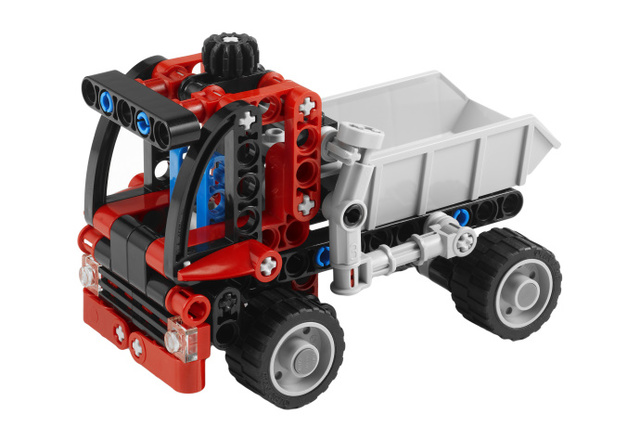
\includegraphics[height=2.1in]{pgloader.jpg}
  \end{center}
\end{frame}

\begin{frame}
  \frametitle{pgloader : Open Source, github}

  \center{\url{https://github.com/dimitri/pgloader}}

  \begin{center}
    
\includegraphics[height=2.1in]{Octocat.png}
  \end{center}
\end{frame}

\begin{frame}
  \frametitle{pgloader : Load Data}

  \center{\url{http://pgloader.io/}}

  \begin{center}
    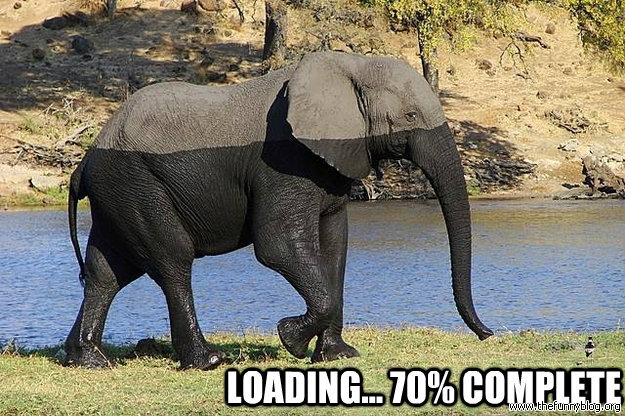
\includegraphics[height=2.1in]{elephant-loading.jpg}
  \end{center}
\end{frame}

\begin{frame}
  \frametitle{From CSV Files}

  \center{\url{http://pgloader.io/howto/csv.html}}

  \begin{center}
    
\includegraphics[height=2.1in]{csv_text.png}
  \end{center}
\end{frame}

\begin{frame}
  \frametitle{From dBase III Files}

  \center{\url{http://pgloader.io/howto/dBase.html}}

  \begin{center}
    
\includegraphics[height=2.1in]{dBase.png}
  \end{center}
\end{frame}

\begin{frame}
  \frametitle{From SQLite}

  \center{\url{http://pgloader.io/howto/sqlite.html}}

  \begin{center}
    
\includegraphics[height=2.1in]{SQLite.png}
  \end{center}
\end{frame}

\begin{frame}
  \frametitle{From a MySQL connection string}

  \center{\url{http://pgloader.io/howto/mysql.html}}

  \begin{center}
    
\includegraphics[height=2.1in]{postgresql_versus_mysql.jpg}
  \end{center}
\end{frame}

\begin{frame}
  \frametitle{From a MySQL connection string}

  \center{\url{http://pgloader.io/howto/mysql.html}}

  \begin{center}
    
\includegraphics[height=2.1in]{mysql.png}
  \end{center}
\end{frame}

\begin{frame}
  \frametitle{pgloader: Transforming data on the fly}

  \center{\url{http://pgloader.io/}}

  \begin{center}
    
\includegraphics[height=2.1in]{huge-full-outer-join.jpg}
  \end{center}
\end{frame}

\begin{frame}
  \frametitle{pgloader version 3.1.0 is now available}

  \begin{center}
    
\includegraphics[height=2.1in]{lisp-python.png}
  \end{center}

  \center{Version 1 \textbf{TCL}, version 2 \textbf{Python},
    version 3 \textbf{Common Lisp}}
\end{frame}

\begin{frame}
  \frametitle{pgloader: loading data \textbf{fast}}

  \begin{center}
    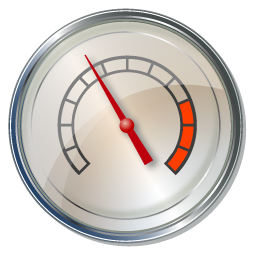
\includegraphics[height=2.1in]{performance-index-00.png}
  \end{center}
\end{frame}

\begin{frame}[fragile]
  \frametitle{User feedback comparing versions 2 and 3, loading CSV files}

  \begin{minted}{postgresql}
 select rows, v2, v3,
        round((  extract(epoch from v2)
        / extract(epoch from v3))::numeric, 2)
        as speedup
   from timing;
        
  rows   |        v2         |       v3        | speedup 
---------+-------------------+-----------------+---------
 4768765 | @ 37 mins 10.878  | @ 1 min 26.917  |   25.67
 3115880 | @ 36 mins 5.881   | @ 1 min 10.994  |   30.51
 3865750 | @ 33 mins 40.233  | @ 1 min 15.33   |   26.82
 3994483 | @ 29 mins 30.028  | @ 1 min 18.484  |   22.55
(4 rows)
  \end{minted}
\end{frame}

\begin{frame}
  \frametitle{\texttt{COPY}}

  \center{The \texttt{copy} command will always be faster than pgloader, but
    has very limited error handling capability.}
  
  \begin{center}
    
\includegraphics[height=1.6in]{rollback-wordmark.png}
  \end{center}
\end{frame}

\begin{frame}[fragile]
  \frametitle{pgloader main features}

  \center{\textit{pgloader} is not just \texttt{copy}}
  \vfill
  
  \begin{itemize}
  \item Error handling with reject files
  \item Transforming data on the fly
  \item A full command language to specify the data loading
  \item Parallel processing architecture allowing async IO
  \item Large number of input file formats, and growing!
  \end{itemize}
  
\end{frame}

\begin{frame}[fragile]
  \frametitle{Setup used to look like an \texttt{INI} file}

  \begin{minted}{ini}
[pgsql]
base = pgloader
client_encoding = 'latin1'
pg_option_standard_conforming_strings = on
null         = ""
empty_string = "\ "
    
[csv]
table            = csv
format           = csv
filename         = csv/csv.data
field_size_limit = 512kB
field_sep        = ,
quotechar        = "
columns          = x, y, a, b, d:6, c:5
only_cols        = 3-6
skip_head_lines  = 1
truncate         = True
  \end{minted}
\end{frame}

\begin{frame}[fragile]
  \frametitle{Now the setup is a \textit{command}}

  \begin{verbatim}
LOAD CSV
     FROM inline (x, y, a, b, c, d)
     INTO postgresql:///pgloader?csv (a, b, d, c)

     WITH truncate,
          skip header = 1,
          fields optionally enclosed by '"',
          fields escaped by double-quote,
          fields terminated by ','

      SET client_encoding to 'latin1',
          work_mem to '12MB',
          standard_conforming_strings to 'on'
  \end{verbatim}
\end{frame}

\begin{frame}[fragile]
  \frametitle{\textit{and the command continues}}

  \begin{verbatim}
   BEFORE LOAD DO
    $$ drop table if exists csv; $$,
    $$ create table csv (
        a bigint,
        b bigint,
        c char(2),
        d text
       );
    $$;
  \end{verbatim}
\end{frame}

\begin{frame}[fragile]
  \frametitle{Examples of supported data sources}

  \begin{verbatim}
  FROM stdin
  FROM inline (a, b, c)
  FROM data/2013_Gaz_113CDs_national.txt
  
  FROM FILENAME MATCHING ~/GeoLiteCity-Location.csv/
  FROM ALL FILENAMES MATCHING ~/F[A-Z]{4}1[45]|OZ20/
  
  FROM http://www.census.gov/geo/maps-data/
              data/docs/gazetteer/places2k.zip
  
  FROM http://www.insee.fr/fr/methodes/nomenclatures/
              cog/telechargement/2013/dbf/historiq2013.zip

  FROM 'sqlite/sqlite.db'              
  FROM mysql://root@localhost/sakila
  FROM mysql://root@unix:/tmp/mysql.sock:/goeuro

\end{verbatim}
\end{frame}

\begin{frame}
  \frametitle{pgloader : Transforming data on the fly}

  \center{\url{http://pgloader.io/}}

  \begin{center}
    
\includegraphics[height=2.1in]{huge-full-outer-join.jpg}
  \end{center}
\end{frame}

\begin{frame}[fragile]
  \frametitle{Transforms}

  \begin{verbatim}
FROM FILENAME MATCHING ~/GeoLiteCity-Blocks.csv/
     WITH ENCODING iso-8859-1
     (
        startIpNum, endIpNum, locId
     )
INTO postgresql:///ip4r?geolite.blocks
     (
        iprange ip4r using (ip-range startIpNum endIpNum),
        locId
     )
  \end{verbatim}
\end{frame}

\begin{frame}[fragile]
  \frametitle{Transforms}

  \begin{verbatim}
FROM FILENAME MATCHING ~/GeoLiteCity-Location.csv/
     (
        locId, country,
        region     null if blanks,
        city       null if blanks,
        postalCode null if blanks,
        latitude, longitude,
        metroCode  null if blanks,
        areaCode   null if blanks
     )
INTO postgresql:///ip4r?geolite.location
     (
        locid, country, region, city, postalCode,
        location point
           using (format nil "(~a,~a)" longitude latitude),
        metroCode, areaCode
     )
  \end{verbatim}
\end{frame}

\section{MySQL}

\begin{frame}
  \frametitle{Full MySQL to PostgreSQL migration in one command}

  \center{\url{http://www.galaxya.fr/}}
  
  \begin{center}
    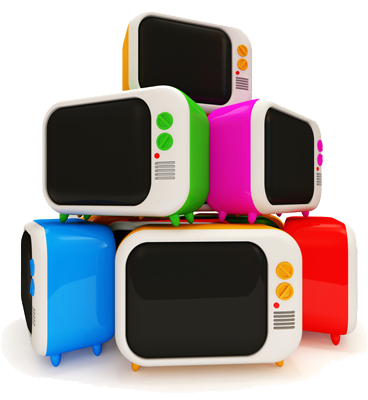
\includegraphics[height=2.1in]{tv.png}
  \end{center}
\end{frame}

\begin{frame}[fragile]
  \frametitle{Working with Galaxya, used previous toolset}
  
  \center{None of them are solving the actual (data) problems...}
  \vfill

  \begin{itemize}
  \item \texttt{mysql2pgsql}, then manually edit the schema
  \item \texttt{SELECT INTO OUTFILE} server side, then \texttt{COPY}
  \item MySQL client pretends to be able to output CSV...
  \item There's always that last \texttt{awk} or \texttt{sed} step
  \item Some ruby and python scripts exist too
  \end{itemize}  
\end{frame}

\begin{frame}
  \frametitle{MySQL vision of data types}

  \center{Empty string and \texttt{NULL}, default values, zero dates
    \texttt{0000-00-00}, \texttt{int(11)}, \texttt{float(20,2)},
    \texttt{tinyint} rather than \texttt{boolean}, \texttt{sets}, encoding,
    ... }
  
  \begin{center}
    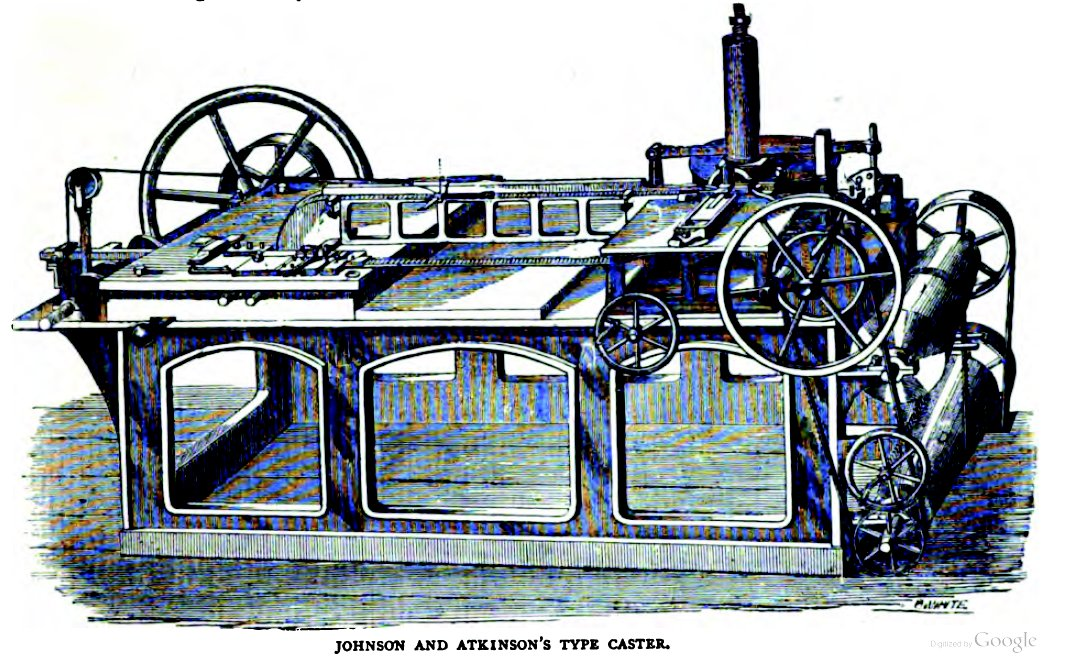
\includegraphics[height=2.1in]{type-casting-machine.jpg}
  \end{center}
\end{frame}

\begin{frame}[fragile]
  \frametitle{MySQL: CAST rules}

\begin{verbatim}
LOAD DATABASE
     FROM      mysql://root@unix:/tmp/mysql.sock:/goeuro
     INTO postgresql://dim@unix:/tmp:/godollar

CAST type datetime to timestamptz
                 drop default drop not null
                using zero-dates-to-null,

     column bools.a to boolean drop typemod
                 using tinyint-to-boolean,

     type char when (= precision 1)
       to char keep typemod,

     column enumerate.foo
      using empty-string-to-null
\end{verbatim}
\end{frame}

\begin{frame}[fragile]
  \frametitle{MySQL: MATERIALIZE VIEWS}

  \center{So that it's possible to change the Schema (DDL) while migrating}
  \vfill
  
\begin{verbatim}
 MATERIALIZE VIEWS foo,
   d as $$
       select cast(d as date) as d, count(*) as n
         from plop
        where d > '2013-10-02'
     group by cast(d as date);
   $$
\end{verbatim}
\end{frame}

\begin{frame}[fragile]
  \frametitle{pgloader limits}
  
  \center{Still quite some work ahead}
  \vfill

  \begin{itemize}
  \item Full support for views (it's another SQL dialect entirely)
  \item Triggers
  \item Stores Procedures
  \item Some data types (geometric)
  \item \texttt{ON UPDATE CURRENT\_TIMESTAMP}
  \end{itemize}  
\end{frame}


\begin{frame}
  \frametitle{Other full database source types}

  \begin{columns}[c]
    \column{.4\textwidth} 
    \begin{center}
      
\includegraphics[height=1.4in]{dBase.png}
    \end{center}

    \column{.6\textwidth} 
    \begin{center}
      
\includegraphics[height=1.4in]{SQLite.png}
    \end{center}
  \end{columns}
\end{frame}

\section{Avenir}

\begin{frame}
  \frametitle{Future}

  \begin{center}
    
\includegraphics[height=2.1in]{avenir.jpg}
  \end{center}
\end{frame}

\begin{frame}
  \frametitle{New data sources}

  \center{Normalizing data while loading might be possible}
  
  \begin{columns}[c]
    \column{.5\textwidth}
    \begin{center}
      
\includegraphics[height=9em]{xml.png}
    \end{center}
    \column{.5\textwidth}
    \begin{center}
      
\includegraphics[height=9em]{logo-json.png}
    \end{center}
  \end{columns}
\end{frame}

\begin{frame}
  \frametitle{Supporting new connection types}

  \begin{columns}[c]
    \column{.5\textwidth}
    \begin{center}
      
\includegraphics[height=4em]{oracle-logo.png}
    \end{center}
    \column{.5\textwidth}
    \begin{center}
      
\includegraphics[height=2em]{Informix_d1323_450x450.png}
    \end{center}
  \end{columns}
  \vfill

  \begin{columns}[c]
    \column{.5\textwidth} 
    \begin{center}
      
\includegraphics[height=4em]{mssql.png}
    \end{center}
    \column{.5\textwidth}
    \begin{center}
      
\includegraphics[height=3em]{sybase_logo.png}
    \end{center}
  \end{columns}
\end{frame}

\section{Conclusion}

\begin{frame}[fragile]
  \begin{center}
    
\includegraphics[height=18em]{free-our-open-data.jpg}
  \end{center}
\end{frame}

\begin{frame}
  \frametitle{Questions?}

\begin{center}
  Now is the time to ask!
  \vfill

  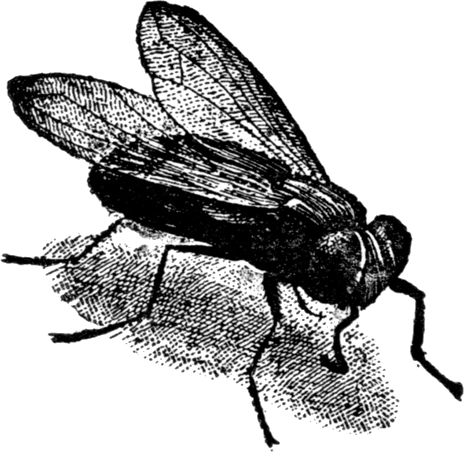
\includegraphics[height=9em]{fly.png}
\end{center}
\end{frame}

\end{document}
